\documentclass[11pt,a4paper,twoside,pdf]{article}

% Paquetes (añade otros si los necesitas):
\usepackage{latexsym}
\usepackage[utf8x]{inputenc}
\usepackage{soul}
\usepackage{array}
\usepackage{amsmath}
\usepackage{amssymb}
\usepackage{marvosym}
\usepackage{epsfig}
\usepackage{graphics}
\usepackage{amsfonts}
\usepackage{xspace}
\usepackage{color}
\usepackage{booktabs}
\usepackage{xtab}
\usepackage{siunitx}
\usepackage{float}
\usepackage{pdfpages}
\usepackage[colorlinks=true,urlcolor=blue,linkcolor=blue,citecolor=blue]{hyperref}
\numberwithin{equation}{section}

% Fuente: palatino
\usepackage[sc]{mathpazo}
\linespread{1.05}

% TFG en inglés:
%\usepackage[english]{babel} 
%\addto\captionsenglish{\renewcommand{\chaptername}{}}

% TFG en español:
\usepackage[spanish,es-nodecimaldot,es-tabla,es-lcroman,es-nosectiondot,
            es-noindentfirst]{babel}
\renewcommand\spanishchaptername{}

% Formato de la página:
\usepackage{fancyhdr}
\usepackage[top=2.88cm,bottom=2.97cm,left=2.95cm,right=2.95cm]{geometry}
\setlength{\parskip}{0.1cm}

% Pon aquí tus definiciones:

\newcommand{\dis}{\displaystyle}
\sodef\an{}{.2em}{1em plus1em}{2em plus.1em minus.1em}

\begin{document}

% Portada %%%%%%%%%%%%%%%%%%%%%%%%%%%%%%%%%%%%%%%%%%%%%%%%%%%%%%%%%%%%%%%%%%%%%%

\pagestyle{empty}


\noindent
\begin{tabular}{r}

\includegraphics[width=8.8cm]{escudoUGRmonocromo.png} \\[-1.8ex]
\hspace{31mm}\vspace{-8mm}
\begin{tabular}{c}
\hline\\[-1ex]\hskip-2mm
{\bf Facultad de Ciencias}\hspace{18mm}
\end{tabular}
\end{tabular}

{\large
\vspace{30mm}
\hspace{25mm}
\begin{tabular}{l}
\an{GRADO EN F\'ISICA}
\end{tabular}

\vspace{45mm}
\hspace{25mm}
\begin{tabular}{l}
\an{TRABAJO FIN DE GRADO}
\\[1.5ex]
\an{\LARGE\bf IMPLEMENTACI\'ON DE }
\\
\an{\LARGE\bf M\'ETODOS}
\\
\an{\LARGE\bf EN DIFERENCIAS FINITAS }
\\
\an{\LARGE\bf EN GPUs}
\end{tabular}

\vfill
\hspace{25mm}
\begin{tabular}{l}
Presentado por:
\\
{\bf D. JUAN JOS\'E SALAZAR L\'OPEZ}
\\[3ex]
Curso Académico 2021/2022
\end{tabular}
}


\newpage

\begin{center}

{\bf Resumen}
\bigskip

\begin{minipage}{0.8\linewidth}
En el siguiente TFG se procede a presentar las ventajas de aplicar el método de diferencias finitas en el dominio del tiempo (FDTD) en GPU, a diferencia del modo de aplicación usual el cual se lleva a cabo usando la potencia de cálculo de las CPUs. La principal diferencia radica en el poder de paralelización de las GPUs, el cual nos proporciona al implementar el método en $\mathbb R^{2}$, una disminución en el tiempo de cálculo de las ecuaciones de Maxwell de aproximadamente un orden de magnitud.

\end{minipage}

\vfill

{\bf Abstract} 
\bigskip

\begin{minipage}{0.8\linewidth}
In the following TFG it is shown the advantages of implementing the finite difference time domain method (FDTD) in GPU, instead of using the calculus power of CPUs. The principal difference is the parallelization power of the GPUs which allows us to decrease the calculus time to solve the Maxwell equations in about one order of magnitude when we implement the method in $\mathbb R^{2}$.
\end{minipage}

\vfill

\end{center}

% Indice %%%%%%%%%%%%%%%%%%%%%%%%%%%%%%%%%%%%%%%%%%%%%%%%%%%%%%%%%%%%%%%%%%%%%%%
\newpage

\tableofcontents

% Texto %%%%%%%%%%%%%%%%%%%%%%%%%%%%%%%%%%%%%%%%%%%%%%%%%%%%%%%%%%%%%%%%%%%%%%%%
\newpage

\pagestyle{fancy}
\fancyhead[RO,LE]{\leftmark}
\fancyhead[LO,RE]{\thepage}
\fancyfoot{}

\section{Introducción}
El método numérico de las diferencias finitas es usado en muchos campos para la resolución de ecuaciones diferenciales de primer orden. En particular, el método de la diferencia central finita cobra especial importancia en la electrodinámica computacional, donde se emplea para resolver las ecuaciones de Maxwell en el dominio del tiempo, discretizando tiempo y espacio para poder implementar la solución en un algoritmo.


Actualmente su uso está muy extendido ya que posibilita el estudio de la propagación de señales electromagnéticas por diversos medios, permitiendo así determinar la propagación de ondas de baja frecuencia (elf) alrededor de la tierra \cite{Taflove2002} o analizar la propagación de ondas electromagnéticas en medios no lineales \cite{Goorjian1991}. En ambos casos se puede aplicar el método conociendo las fuentes de la radiación y las propiedades del medio que se desea estudiar. También es de interés su estudio en la construcción de antenas, ya que conociendo la topologia de las fuentes se pueden crear modelos para determinar la propagación de las ondas generadas. En concreto, el método ha sido necesario para el estudio de la radiación generada por antenas de tipo bocina \cite{Taflove1991}.

Así mismo, el método no solo se utiliza en electrodinámica computacional, también es de especial interés en ingeniería biomédica, donde permite la investigación de nuevas formas de detección de cancer de mama utilizando ondas de microondas en lugar de rayos X o ultrasonido \cite{Taflove1998}.

Desde que se desarrolló el método y se generaron los primero algoritmos hasta ahora se ha hecho uso del poder de cómputo que nos proporcionan las CPUs, el cual ha ido creciendo con el paso de los años. No obstante, con el aumento de las dimensiones del problema a resolver, también aumenta el tiempo necesario para obtener la solución de las ecuaciones. Esto es debido a la forma usual de implementación del método, la cual se basa en calcular los valores del campo punto a punto de forma secuencial, aumentando así el tiempo de cálculo proporcionalmente con las dimensiones del problema.

  Esta situación puede solventarse haciendo uso del poder de paralelización que nos ofrecen las tarjetas gráficas (GPUs), pudiendo paralelizar hasta cierto límite, todas las operaciones necesarias en cada coordenada de la dimensión espacial gracias a la arquitectura con la que están creadas. Estos dispositivos están compuestos por miles de microprocesadores, pudiendo realizar cálculos en cada uno de ellos simultaneamente. Para poder utilizar el poder de paralelización de las GPUs es necesario utilizar CUDA, lenguaje de programación desarrolado por Nvidia basado en C, el cual nos permite seleccionar un número concreto de microprocesadores generalmente acorde a las dimensiones del problema, permitiendonos reducir así el tiempo empleado en realizar los cálculos.








\section{Metodología}
\subsection{El método de diferencias finitas en el dominio del tiempo} \label{section:metodo_diferencias_finitas}
El método numérico de las diferencias finitas se emplea en la resolución de ecuaciones diferenciales de primer orden, en particular, el método de la diferencia central finita se basa en aproximar de forma sencilla la derivada de una función en un punto como la diferencia de dicha función evaluada en dos puntos equidistantes al mismo. Haciendo uso del desarrollo en serie de Taylor y aproximando a tercer orden obtenemos:

\begin{equation}
f(x+h)=y(x)+hy^\prime(x)+\frac{h^3}{2}y^{\prime\prime}(x)+\frac{h^3}{6}y^{\prime\prime\prime}(x)
\end{equation}

\begin{equation}
f(x-h)=y(x)-hy^\prime(x)+\frac{h^3}{2}y^{\prime\prime}(x)-\frac{h^3}{6}y^{\prime\prime\prime}(x)
\end{equation}

\begin{equation}
y\prime(x)=\frac{y(x+h)-y(x-h)}{2h}+O(h^2)
\end{equation}

Donde hemos despejado el valor de la derivada de la función en un punto mediante su desarrollo en serie en $(x+h)$ y $(x-h)$.

Recordando la expresión de las ecuaciones de Maxwell para el campo electromagnético, haciendo uso del vector campo $D$.

\begin{equation}
\frac{\partial D}{\partial t}=\nabla \times H
\end{equation}

\begin{equation}
\frac{\partial H}{\partial t}=-\frac{1}{\mu_{0}}\nabla \times E
\end{equation}

\begin{equation}
D(\omega)=\varepsilon_{0}\varepsilon^*_{r}(\omega)E(\omega)
\end{equation}

Podemos observar que están expresadas en el dominio de la frecuencia para poder aplicarlas a medios cuya constante dieléctrica dependa de la misma. Resaltar que $\varepsilon_{0}$ y $\varepsilon_{r}$ corresponden con las constantes dieléctricas del vacío y del medio respectivamente, y $\mu_{0}$ es la permeabilidad magnética del vacío.


Para simplificar el formalismo es conveniente normalizar las ecuaciones haciendo uso de las constantes dieléctrica y permeabilidad magnética del vacío.
\begin{equation}
\tilde{E}=\sqrt{\frac{\varepsilon_{0}}{\mu_{0}}}E
\end{equation}

\begin{equation}
\tilde{D}=\frac{1}{\sqrt{\varepsilon_{0}\mu_{0}}}D
\end{equation}

De este modo podemos expresar las ecuaciones de Maxwell para el campo electromagnético como:

\begin{equation}
\frac{\partial \tilde{D}}{\partial t}=-\frac{1}{\sqrt{\varepsilon_{0}\mu_{0}}}\nabla \times H
\end{equation}

\begin{equation}
\frac{\partial H}{\partial t}=-\frac{1}{\sqrt{\varepsilon_{0}\mu_{0}}}\nabla \times E
\end{equation}

\begin{equation}
\tilde{D}(\omega)=\varepsilon^*_{r}(\omega)\tilde{E}(\omega)
\end{equation}


En $\mathbb R^{3}$ tenemos 3 componentes para el campo eléctrico y 3 para el magnético $\tilde{E}_{x}$, $\tilde{E}_{y}$, $\tilde{E}_{z}$, $H_{x}$, $H_{y}$, $H_{z}$, por lo que, si queremos aplicar un modelo en dos dimensiones debemos elegir uno de los dos grupos de tres vectores, (i) el transversal magnético, formado por $\tilde{E}_{z}$, $H_{x}$, $H_{y}$, o (ii) el transversal eléctrico, compuesto por los vectores $\tilde{E}_{x}$, $\tilde{E}_{y}$ y $H_{z}$.

Usaremos el modo transversal magnético y utilizaremos directamente las letras E y D sin tildar para nombrar a las componentes normalizadas de los campos:

\begin{equation}
\frac{\partial D_{z}}{\partial t}=\frac{1}{\sqrt{\varepsilon_{0}\mu_{0}}}(\frac{\partial H_{y}}{\partial x}-\frac{\partial H_{x}}{\partial y})
\end{equation}

\begin{equation}
{D}(\omega)=\varepsilon^*_{r}(\omega)E(\omega)
\end{equation}

\begin{equation}
\frac{\partial H_{x}}{\partial t}=-\frac{1}{\sqrt{\varepsilon_{0}\mu_{0}}}\frac{\partial E_{z}}{\partial y}
\end{equation}

\begin{equation}
\frac{\partial H_{y}}{\partial t}=\frac{1}{\sqrt{\varepsilon_{0}\mu_{0}}}\frac{\partial E_{z}}{\partial x}
\end{equation}

Estas son las ecuaciones de una onda plana moviéndose en la dirección $x$ e $y$ con el campo eléctrico orientado en la dirección $z$ y el magnético en las direcciones $x$ e $y$. Las componentes a calcular son ecuaciones diferenciales de primer orden, por lo que, aplicando el método de la diferencia central finita componente a componente obtenemos:

\begin{equation}
\begin{split}
\frac{D^{n+1/2}_{z}(i,j)-D^{n-1/2}_{z}(i,j)}{\Delta t}=\frac{1}{\sqrt{\varepsilon_{0}\mu_{0}}}\left[\frac{H^{n}_{y}(i+\frac{1}{2},j)-H^{n}_{y}(i-\frac{1}{2},j)}{\Delta x}\right]  \\
-\frac{1}{\sqrt{\varepsilon_{0}\mu_{0}}}\left[\frac{H^{n}_{x}(i,j+\frac{1}{2})-H^{n}_{x}(i,j-\frac{1}{2})}{\Delta x}\right] 
\end{split}
\end{equation}

\begin{equation}
\frac{H^{n+1}_{x}(i,j+\frac{1}{2})-H^{n}_{x}(i,j+\frac{1}{2})}{\Delta t}=-\frac{1}{\sqrt{\varepsilon_{0}\mu_{0}}}\left[\frac{E^{n+1/2}_{z}(i,j+1)-E^{n+1/2}_{z}(i,j)}{\Delta x}\right] 
\end{equation}

\begin{equation} 
\frac{H^{n+1}_{y}(i+\frac{1}{2},j)-H^{n}_{y}(i+\frac{1}{2},j)}{\Delta t}=\frac{1}{\sqrt{\varepsilon_{0}\mu_{0}}}\left[\frac{E^{n+1/2}_{z}(i+1,j)-E^{n+1/2}_{z}(i,j)}{\Delta x}\right] 
\end{equation}

En estas ecuaciones el tiempo se especifica con el superíndice, donde n es el paso temporal, de modo que $t=\Delta t\cdot n$. En los paréntesis utilizamos los valores de i, j para determinar la posición, sin olvidar que el campo eléctrico y el magnético están intercalados en tiempo y espacio, lo cual se especifica con la suma y resta de valores $\frac{1}{2}$ en los superíndices y paréntesis. En la figura \ref{fig:EyH_intercalados} se muestra el intercalado de los campos en el espacio.

\begin{figure}[h]
\centering
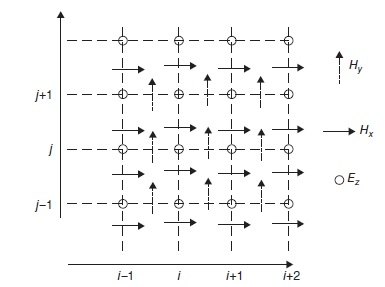
\includegraphics[width=10cm]{Interleaving_E_H.jpg}				
\caption{Campos Ez, Hx y Hy intercalados \cite{Houle2020}. }
\label{fig:EyH_intercalados}
\end{figure}
\noindent

Utilizaremos $\Delta x = \Delta y$, por lo que al haber elegido el tamaño de celda ($\Delta x \cdot \Delta y$), podemos calcular el salto temporal como:

\begin{equation}
\Delta t=\frac{\Delta x}{2 \cdot c_{0}}
\end{equation}

Donde $c_{0}$ es la velocidad de la luz en el vacío. Recordando que $\varepsilon_{0} \mu_{0}=1/(c_{0})^2$ y teniendo en cuenta la normalización utilazada:

\begin{equation}
    \frac{\Delta t}{\sqrt{\varepsilon_{0} \mu_{0}} \Delta x}=\frac{\Delta x}{2 \cdot c_{0}}\cdot 
     \frac{1}{\sqrt{\varepsilon_{0} \mu_{0}} \Delta x}=\frac{1}{2}
\end{equation}

Lo que nos permite, junto a las expresiones discretizadas en tiempo y espacio de las ecuaciones de Maxwell y la normalización empleada, generar un algoritmo de forma sencilla para calcular los campos:

\begin{align} \label{eq:actualizacion-campos}
    dz[i,j]&=dz[i,j] + 0.5*(hy[i,j]-hy[i-1,j]-hx[i,j]+hx[i,j-1]) \nonumber \\
    ez[i,j]&=gaz[i,j]*dz[i,j] \nonumber \\
    hx[i,j]&=hx[i,j]+0.5*(ez[i,j]-ez[i,j+1]) \nonumber \\
    hy[i,j]&=hy[i,j]+0.5*(ez[i+1,j]-ez[i,j])
\end{align}

El valor $gaz[i,j]$ depende de las características del medio, por lo que si suponemos vacío su valor es 1. De este modo las ecuaciones \eqref{eq:actualizacion-campos} corresponden a los vectores necesarios para determinar los campos en $\mathbb R^{2}$, donde solo es necesario conocer el valor de la fuente que genera la radiación, ya sea de cualquier tipo, sinusoidal o un pulso entre otros.  

En general, para conocer el valor del campo en todo el espacio es necesario calcular  su componente punto a punto pero utilizando la paralelización de la GPU podemos calcularlos todos los valores de los vectores a la vez.



\subsection{GPU} \label{subsection:GPU}

A lo largo de los años, debido a la necesidad de procesar gráficos de alta definición al instante, las tarjetas gráficas se han convertido en sistemas multinúcleo con la capacidad de multiproceso paralelizado. Las unidades de procesamiento de gráficos (GPUs) proporcionan más rendimiento y ancho de banda de memoria que las CPUs al mismo precio. Muchas aplicaciones aprovechan esta ventaja para ejercutarse más rapido en GPU que en CPU. La diferencia de potencia de las GPUs y las CPUs se basa en el propósito para el que fueron diseñadas las mismas. Las CPUs se crearon para que, con los pocos núcleos con que se construyen, ejecuten cálculos de forma secuencial en el menor tiempo posible. No obstante, las GPUs se crearon con miles de núcleos para que trabajen todos a la vez, realizando todos los cálculos paralelamente en vez de usar una metodología secuencial.

En la figura \ref{fig:arquitectura-cpu-gpu} se muestra la diferencia de estructura entre CPU y GPU, variando la cantidad de núcleos de la misma según el modelo de dispositivos utilizados. En general, dada la necesidad de ejecutar procesos tanto secuenciales como paralelos los sistemas están diseñados para poder mezclar los atributos de las CPUs y las GPUs maximizando así el rendimiento de los algoritmos \cite{web}.

\begin{figure}[h]
\centering
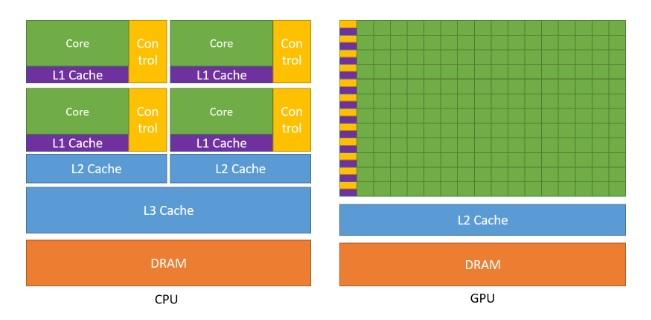
\includegraphics[width=15cm]{Nvidia-CPU-GPU.jpg}				
\caption{Diferencia de transistores entre CPU y GPU \cite{web}. }
\label{fig:arquitectura-cpu-gpu}
\end{figure}
\noindent

Nvidia ha desarrollado CUDA para generar soluciones que utilicen la paralerización de las tarjetas gráficas, un lenguaje de programación basado en C, el cual comparte sintaxis en muchos aspectos con este último. En CUDA distinguimos dos tipos de procesos, los llevados a cabo en la CPU (host) y los ejecutados desde la GPU (Device o Kernel), teniendo acceso ambos dispositivos a dos tipos de memoria, llamadas global y constante. En la figura \ref{fig:componentes gpu} se muestra la estructura del device y cómo ambos comparten dichas memorias. Para identificar el lugar de ejecución de cada función en CUDA se especifica en el encabezado de la misma las palabras \_\_host\_\_ en las aplicaciones ejecutadas en CPU y \_\_global\_\_ en las ejecutadas en GPU.

Cada tarjeta gráfica tiene un número determinado de threads o hilos, los cuales pueden realizar un cálculo concreto simultáneamente cuando son llamados por una función global (desde el device). Para realizar esta llamada CUDA divide los núcleos en bloques y mallas como se puede ver en la figura \ref{fig:componentes gpu}, donde se muestra una malla de dos bloques y dos hilos en cada bloque, siendo 4 los hilos totales. Destacar que en general el número de hilos tiene que coincidir necesariamente con el número de núcleos ya que, como ocurre en las CPUs, puede haber varios hilos en un mismo núcleo. Esto significa que dentro de un mísmo núcleo pueden realizarse tantos cálculos simultáneos como hilos tenga dicho procesador, no obstante la diferencia de hilos entre un procesador y una gráfica es de varios órdenes de magnitud, pudiendo ser 6 en una CPU y miles en una GPU.

\begin{figure}[h]
\centering
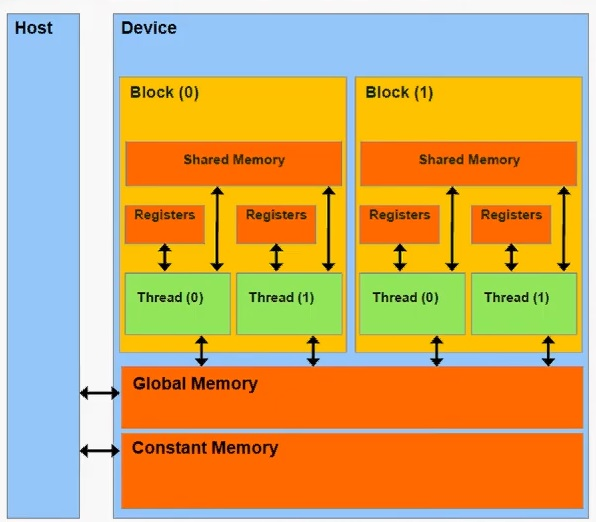
\includegraphics[width=10 cm]{Nvidia-Device_Structure.jpg}				
\caption{Estructura del Host (\cite{web}). }
\label{fig:componentes gpu}
\end{figure}
\noindent

Al implementar una solución, desde el host se selecciona el número de hilos a utilizar teniendo en cuenta las limitaciones de hilos por bloques y bloques por mallas de la tarjeta gráfica que se esté utilizando y desde la función global (en el device) se determinan las operaciones a realizar por cada hilo. Es decir, antes de ejecutar la función \_\_globla\_\_ se debe conocer el número de hilos y bloques a utilizar por la GPU, pudiendo lanzar un número determinado de estos en las tres dimensiones del espacio (x,y,z).

Dadas las variables a utilizar, hilos, bloques y mallas, es necesario identificar el hilo que se quiere utilizar para ejecutar el cálculo. Conceptualmente podemos ver una malla como una matriz, dividida por bloques e hilos dentro de estos bloques como se muestra en la figura \ref{fig:hilos, bloques y mallas en gpu}. En ella podemos ver una malla compuesta por 60 hilos, dividida por 4 bloques, dos en la dimensión x denotada por 'gridDim.x', dos en la dimensión y denotada por 'gridDim.y', estando cada bloque compuesto de 15 hilos.

\begin{figure}[h]
\centering
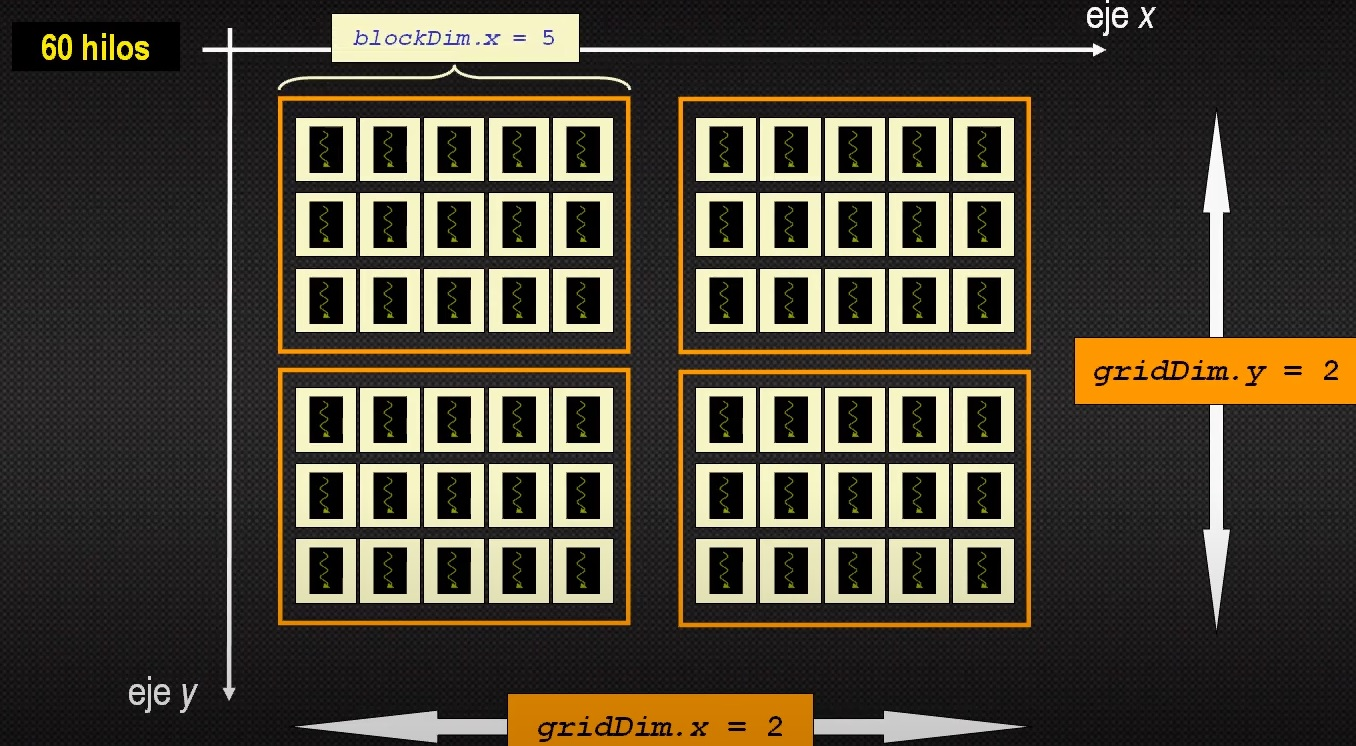
\includegraphics[width=10 cm]{Nvidia_Topologia_virtual.jpg}				
\caption{Topología dentro de hilos, bloques y mallas \cite{web} }
\label{fig:hilos, bloques y mallas en gpu}
\end{figure}
\noindent

No obstante, en CUDA esta división es lineal como se muestra en la figura \ref{fig:localizacion de hilos}. En ella podemos ver separados por franjas claras y oscuras el paso de un bloque a otro, estando estos divididos por el número de hilos que hay dentro de cada bloque. De modo que, para poder identificar un hilo podemos concebir la malla como una matriz donde las filas determinan el bloque y las columnas los hilos. Así, se distingue unívocamente cada hilo multiplicando las columnas totales por el número del bloque donde está el hilo y sumandole la posición que ocupa en el.

\begin{figure}[h]
\centering
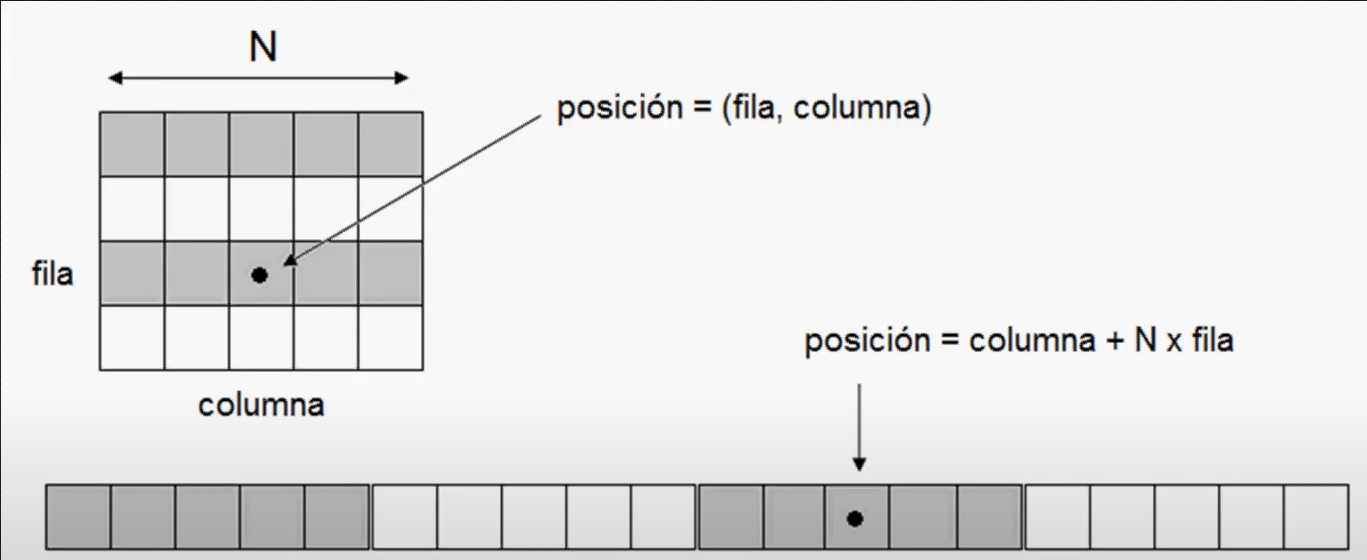
\includegraphics[width=10 cm]{Nvidia_Posicion_hilo.jpg}				
\caption{Identificación de hilo dentro de una malla.}
\label{fig:localizacion de hilos}
\end{figure}
\noindent

En nuesto caso, debido a las necesidades del problema necesitamos identificar los hilos de una malla lanzada con hilos y bloques en dos dimensiones. Por lo que necesitamos identificar qué son las filas y las columnas en nuestra función \_\_globla\_\_. Esta identificación la conseguimos usando las palabras reservadas que nos proporciona CUDA:

\begin{verbatim}
     int fil = blockIdx.y * blockDim.y + threadIdx.y;
     int col = blockIdx.x * blockDim.x + threadIdx.x;
\end{verbatim}

Es necesario resaltar la necesidad de seleccionar la cantidad de hilos y bloques acorde a la capacidad de la gráfica y las necesidades del problema. En específico, para la resolución de las ecuaciones de Maxwell en dos dimensiones para un mallado de un millón de puntos, dividido en 1000 posiciones en la dimensión x y 1000 posiciones en la dimensión y, con la gráfica utilizada en este TFG (la cual perrmite 1024 hilos por bloque), es necesario utilizar un mínimo de 977 bloques de 1024 hilos cada uno.


Finalmente, para medir el tiempo de cálculo en el device CUDA nos proporciona la función 'cudaEvent', con la cual se establecen dos marcas de tiempo en el algoritmo y se calcula el tiempo como la resta de estas mismas, siendo la diferencia el tiempo transcurrido en el device al realizar las operaciones.
Para calcular el tiempo en el host se ha utilizado la función 'clock\_t' y de la misma forma se han creado dos marcas temporales y se ha calculado la diferencia. En ambos casos se han dividido los resultados entre las cuentas por segundo dentro del procesador y la tarjeta gráfica para obtener el tiempo en segundos con una precisión de $\pm \SI{0.001}{\second}$.

\section{Algoritmo}
En este TFG el autor ha desarrollado varios códigos en CUDA de libre uso para la resolución de las ecuaciones de Maxwell aplicando el método FDTD en dos dimensiones. Los códigos generados pueden encontrarse en el siguiente repositorio de github:

\url{https://github.com/juanjo1213/TFG-FDTD}

En el mismo están los algoritmos utilizados para la solución en 2D implementada tanto en la cpu y en la gpu. La implementación de la solución en el device está nombrada como 'fd2d\_simp.cu' y la ejecutada en el host como 'HOST\_FD2D\_SIMP.cu'.



Para la ejecución de los algoritmos se ha utilizado un procesador i7-6700K procesador de 4 núcleos y 8 hilos con una frecuencia máxima de 4.2 GHz por núcleo y una tarjeta gráfica GTX 1070 con 8GB de memoria RAM y un total de 1920 núcleos CUDA. 

A continuación se muestra la función \_\_host\_\_ generada para el cálculo de las ecuaciones \ref{eq:actualizacion-campos}, esta es llamada desde el host y recibe como parámetro un 'struct' que contiene los vectores campo a calcular. En ella se ejecutan varios bucles para el cálculo secuencial de los campos punto a punto y para mayor similitud, se han almacenado las matrices como vectores de dimensión $dimx\cdot dimy$ y se ha determinado cada componente a calcular como se expuso en la sección \ref{subsection:GPU}. 


\begin{verbatim}
void FD2D(FDTDData* field, int xdim, int ydim, int nsteps)
{
 int ic = int(xdim / 2),
  jc = int(ydim / 2);

 //Medium conditions
 double* gaz;

 gaz = (double*)malloc(xdim * ydim * sizeof(double));

 for (int j = 0;j < ydim;j++) {
  for (int i = 0;i < xdim;i++) {
   gaz[j * xdim + i] = 1.0;
  }
 }


 double ddx = 0.01,         //cell size
     dt = ddx / 6e8,     //Time step size
     epsz = 8.854e-12;   //Dielectric profile



 //Pulse parameters
 double t0 = 20.0,
  spread = 6.0;

 //Main loop
 for (int time_step = 1;time_step < nsteps + 1;time_step++)
 {
  //Calculate Dz
  for (int j = 1;j < ydim;j++) {
   for (int i = 1;i < xdim;i++) {
    field[j*xdim+i].dz= field[j * xdim + i].dz+
                        0.5*(field[j*xdim+i].hy- field[j * xdim + i-1].hy-
                        field[j*xdim+i].hx+ field[(j-1) * xdim +i].hx);
   }
  }

  //Gaussian pulse in the middle
  double pulse = exp(-0.5 * 
           ((t0 - time_step) / spread) * ((t0 - time_step) / spread));
  field[jc * xdim + ic].dz = pulse;

  //Calculate the Ez field from Dz
  for (int j = 1;j < ydim;j++) {
   for (int i = 1;i < xdim;i++) {
    field[j * xdim + i].ez = gaz[j * xdim + i] * field[j * xdim + i].dz;
   }
  }

  //Calculate the Hx field
  for (int j = 0;j < ydim-1;j++) {
   for (int i = 0;i < xdim-1;i++) {
    field[j * xdim + i].hx = field[j * xdim + i].hx + 
            0.5 * (field[j * xdim + i].ez - field[(j + 1) * xdim + i].ez);
   }
  }

  //Calculate the Hy field
   //Calculate the Hx field
  for (int j = 0;j < ydim - 1;j++) {
   for (int i = 0;i < xdim - 1;i++) {
    field[j * xdim + i].hy = field[j * xdim + i].hy + 
          0.5 * (field[j * xdim + i + 1].ez - field[j * xdim + i].ez);
   }
  }

 }




}
\end{verbatim}

En el siguiente algoritmo se muestra la función \_\_global\_\_ generada para realizar los cálculos de forma paralela. En ella podemos ver como se determinan las filas y las columnas utilizadas para determinar los hilos a utilizar como se explicó en la sección \ref{subsection:GPU}. La función, al igual que la función anterior, recibe como parámetro un struct que contiene los vectores a calcular, las dimensiones $x$ e $y$ del problema y el paso temporal que se está ejecutando. Al existir la posibilidad de reservar más bloques e hilos de los necesarios para realizar los cálculos, se usa el condicional 'if' para especificar el número de hilos a utilizar.

\begin{verbatim}
    __global__ void FD2D(FDTDData* field, int xdim, int ydim, int ts)
{
 int fil = blockIdx.y * blockDim.y + threadIdx.y;
 int col = blockIdx.x * blockDim.x + threadIdx.x;


 int ic = int(xdim / 2),
  jc = int(ydim / 2);

 double ddx = 0.01,
  dt = ddx / 6e8,
  epsz = 8.854e-12;

 //pulse parameters
 double t0 = 20.0,
  spread = 6.0;

 //Calculate Dz
 if (0 < fil && fil < ydim && 0 < col && col < xdim) {
  field[fil * xdim + col].dz += 0.5 * 
      (field[fil * xdim + col].hy - field[fil * xdim + col - 1].hy -
   field[fil * xdim + col].hx + field[(fil - 1) * xdim + col].hx);
 }
 __syncthreads();

 //Gaussian pulse in the middle
 double pulse = exp(-0.5 * ((t0 - ts) / spread) * ((t0 - ts) / spread));
 field[jc * xdim + ic].dz = pulse;
 __syncthreads();

 //Calculate the Ez field from Dz
 if (0 < fil && fil < ydim && 0 < col && col < xdim) {
  field[fil * xdim + col].ez = field[fil * xdim + col].gaz * 
                               field[fil * xdim + col].dz;
 }
 __syncthreads();

 //Calculate the Hx field
 if (fil < ydim - 1 && col < xdim - 1) {
  field[fil * xdim + col].hx += 0.5 * (field[fil * xdim + col].ez - 
                                     field[(fil + 1) * xdim + col].ez);
 }
 __syncthreads();

 //Calculate the Hy field
 if (fil < ydim - 1 && col < xdim - 1) {
  field[fil * xdim + col].hy += 0.5 * 
        (field[fil * xdim + col + 1].ez - field[fil * xdim + col].ez);
 }

}
\end{verbatim}

En ambas funciones se emplea un bucle ya sea dentro o fuera de la función para especificar el número de pasos temporales a realizar, además de utilizar como fuente de los campos un pulso gaussiano, denotado en ambas funciones como 'pulse' y generado en el centro del espacio.





\section{Resultados}

Al resolver las ecuaciones \ref{eq:actualizacion-campos} obtenemos una onda electromagnética propagándose por el espacio, en nuestro caso, siendo generada por un pulso gaussiano como fuente. La figura \ref{fig:solucion} muestra la propagación del campo eléctrico (Ez) en un espacio de 3600 puntos y 20, 30, 40, 50 pasos temporales. Como podemos ver, la onda generada en el centro del espacio se propaga en las direcciones $x$ e $y$.  

\begin{figure}[ht]
\centering
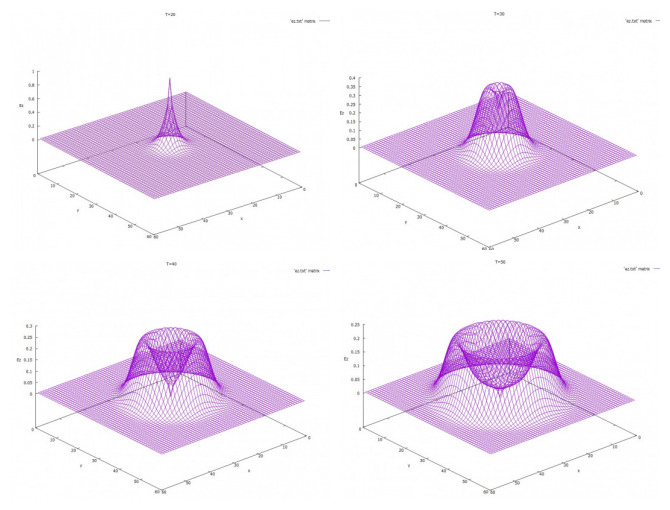
\includegraphics[width=15 cm]{Solution.JPG}				
\caption{Propagación del campo eléctrico en $\mathbb R^{2}$ en un espacio de 3600 puntos en 20 (Superior-Izquierda), 30 (Superior-Derecha), 40 (Inferior-izquierda) y 50 (Inferior-Derecha) pasos temporales.}
\label{fig:solucion}
\end{figure}
\noindent

Para determinar el aumento de velocidad en tiempo de cálculo al implementar este algoritmo en GPU se han realizado dos experimenteos donde se determina su dependencia con el número de pasos temporales y la densidad de puntos. En ambos se han realizado una serie de ejecuciones para cada tiempo a determinar, de las cuales se han calculado el porcentaje de dispersión, la media y se ha elegido el error del resultado como el máximo entre la sensibilidad de la medida y la desviación de la media.

\subsection{Dependencia del tiempo de cálculo con el número de pasos temporales} \label{Subsection:Variacion pasos temporales}

Para determinar la dependencia del tiempo de cálculo con el número de pasos temporales se han llevado a cabo varias ejecuciones en host y device. En estas se ha utilizado una densidad constante de puntos de 25 millones y se han variado los pasos temporales desde 10 hasta 10 000 realizando un mínimo de tres medidas para cada valor de pasos temporales en cada algoritmo. En la tabla  \ref{tab:npasos} se enumeran los datos obtenidos en las ejecuciones realizadas, en ella se ha nombrado al tiempo de ejecución en CPU como $t_\text{CPU}$ y el tiempo de ejecución en el device como $t_\text{GPU}$. En la última columna se ha calculado el llamado aumento de velocidad (speed up) para determinar la mejora en tiempo de ejecución de una tecnología a otra.

Como podemos ver en la tabla, haciendo la media de los valores calculados, obtenemos una mejora en la velocidad de ejecución (speed up) de aproximadamente 12.31 $\pm$ 0.5. Esto nos indica que el algoritmo desarrollado en GPU nos ofrece una solución con un aumento del 12.31 en la velocidad de cálculo que la solución en CPU.

\begin{table}[h]
    \centering
    \begin{tabular}{|r|c|c|c|}
    \hline
    Pasos Temporales &  $t_\text{CPU}$ ($\SI{}{\second}$)  & $t_\text{GPU}$ ($\SI{}{\second}$) &  ($t_\text{GPU}$/$t_\text{CPU}$)  \\ \hline \hline
     10 & 1.971 $\pm$ 0.008 & 0.165 $\pm$ 0.001 & 11.91 $\pm$ 0.09\\ \hline
     100 & 19.32 $\pm$ 0.05 & 1.633 $\pm$ 0.003 & 11.83 $\pm$ 0.04\\ \hline
     1000 & 209.1 $\pm$ 1.4 & 16.397 $\pm$ 0.023 & 12.75 $\pm$ 0.09\\ \hline
     10000 & 2150 $\pm$ 13 & 168.6 $\pm$ 0.9 & 12.75 $\pm$ 0.10\\ \hline
    \end{tabular}
    \caption{Datos obtenidos tras medir la dependencia del tiempo de cálculo con el número de pasos temporales en CPU y GPU además de calcular el aumento en velocidad al usar CUDA.}
    \label{tab:npasos}
\end{table}


Al escoger un aumento lineal del número de pasos temporales cabe esperar que el aumento del tiempo de cálculo también sea lineal, ya que en ambos se ha empleado un bucle para realizar las funciones un número determinado de veces. No obstante, también es de esperar que en el device el tiempo de cálculo sea mucho menor debido a la paralelización aplicada, reduciendo el tiempo que se tarda en pasar de una sección del bucle a otra. Podemos comprobar estos resultados en la figura \ref{fig:t-pasos_temporales}, donde vemos un gráfico de los resultados obtenidos en la tabla \ref{tab:npasos}, representando en color azul los correspondientes al algoritmo ejecutado en el host y en color naranja los del device. En el gráfico se han representado las regresiones lineales obtenidas para las dos series de datos, siguiendo ambas una tendencia completamente lineal ya que en las dos se ha obtenido un valor del coeficiente $R^2$ de 0.99.

Es de interés destacar la diferencia en las pendientes de ambas regresiones, siendo en la del host de 0.2152 $\pm$ 0.0003 $\SI{}{\second}$ y la del device de 0.01687 $\pm$ 3$\cdot 10^{-5}$ $\SI{}{\second}$, lo que nos indica, al ser la pendiente del host de un orden de magnitud mayor que la del device, un aumento mucho menor en el tiempo de cálculo al aumentar el número de pasos temporales utilizando el host que aplicando el algoritmo en la CPU.


\begin{figure}[h]
\centering
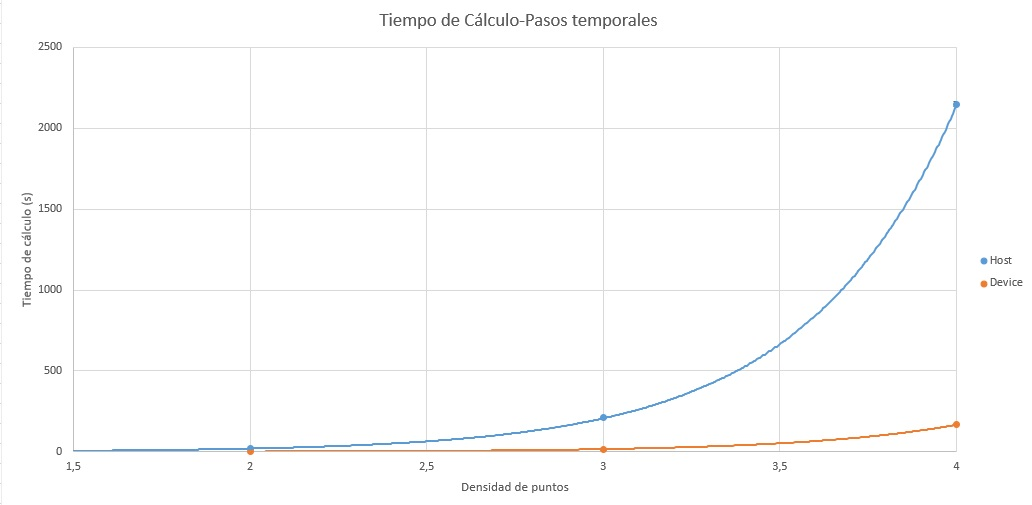
\includegraphics[width=15 cm]{T-Pasos_temporales.jpg}				
\caption{Relación entre el tiempo de cálculo y el número de pasos temporales para una densidad de puntos de 25 millones. La línea naranja representa el tiempo de ejecución en el device y la azul el tiempo de ejecución en el host. En ambas series de datos se ha representado la recta obtenida tras hacer una regresión lineal. Los valores de la pendiente obtenidos son de 0.2152 $\pm$ 0.0003 $\SI{}{\second}$ para el host y de 0.01687 $\pm$ 3$\cdot 10^{-5}$ $\SI{}{\second}$ para el device.}
\label{fig:t-pasos_temporales}
\end{figure}
\noindent






\subsection{Variación del tiempo de cálculo al variar la densidad de puntos} \label{subsection: Variacion densidad de puntos}

Para determinar la dependencia del tiempo  de cálculo de los algoritmos con la densidad de puntos utilizada, también se han realizado varias ejecuciones tanto en host como en device. En todas ellas se ha mantenido constante el número de pasos temporales, 1000 y se ha variado la densidad de puntos desde $10^6$ hasta $25\cdot 10^6$. No se han escogido valores equiespaciados de la densidad de puntos para la recolección de datos por la condición mencionada en la sección \ref{section:metodo_diferencias_finitas}, donde escogimos $\Delta x=\Delta y$ para así facilitar el desarrollo de las expresiones. En la tabla \ref{tab:t_densidad_de_punto} se recogen los datos obtenidos dividos en columnas, al igual que en el apartado anterior, se han utilizado las letras  $t_\text{CPU}$ y  $t_\text{GPU}$ para nombrar a los tiempos de cálculo de host y device respectivamente. 

En la última columna también se recoge el aumento en velocidad de cálculo (speed up), siendo en este caso la media de los valores de 13 $\pm$ 0.9, lo que nos indica que obtenemos una solución en GPU 13 veces más rápido que en CPU.

\begin{table}[h]
    \centering
    \begin{tabular}{|r|c|c|c|}
    \hline
    Densidad de puntos &  $t_\text{CPU}$ ($\SI{}{\second}$)  & $t_\text{GPU}$ ($\SI{}{\second}$) &  ($t_\text{GPU}$/$t_\text{CPU}$)  \\ \hline \hline
     $10^6$ & 7.67 $\pm$ 0.04         & 0.640 $\pm$ 0.002 & 11.98 $\pm$ 0.07\\ \hline
     $4\cdot 10^6$ & 35.36 $\pm$ 0.23 & 2.447 $\pm$ 0.016 & 14.44 $\pm$ 0.13\\ \hline
     $9\cdot 10^6$ & 72.3 $\pm$ 0.3   & 5.582 $\pm$ 0.021   & 12.96 $\pm$ 0.07\\ \hline
     $16\cdot 10^6$ & 126.3 $\pm$ 0.5 & 9.81 $\pm$ 0.03   & 12.88 $\pm$ 0.06\\ \hline
     $25\cdot 10^6$ & 209.1 $\pm$ 1.4 & 16.397 $\pm$ 0.23 & 12.75 $\pm$ 0.09\\ \hline
    \end{tabular}
    \caption{Datos obtenidos tras medir la dependencia del tiempo de cálculo con la densidad de puntos en CPU y GPU además de calcular el aumento de velocidad al usar la GPU.}
    \label{tab:t_densidad_de_punto}
\end{table}


Al igual que el apartado anterior, al aumentar la densidad de punto haciendo el problema un número x de veces más grande cabe esperar algún tipo de tendencia en el tiempo de cálculo para ambos algoritmos, siendo esta tendencia menos pronunciada en el algoritmo CUDA aplicado en GPU. Para determinar este comportamiento, en la figura \ref{fig:t-densidad_de_puntos} se han representado los datos obtenidos en la tabla \ref{tab:t_densidad_de_punto}. En ella se ha realizado una regresión lineal para las dos series de valores (CPU y GPU), deduciendo que los valores se ajustan a una recta al obtener un valor de $R^2$ de 0.99 para ambas. 

Como es de esperar, se obtiene un valor de pendiente mayor para el algoritmo implementado en la CPU, 8.2 $\pm 0.2 \cdot 10^{-6}$, que el calculado en el algoritmo implementado en GPU, 6.52 $\pm 0.16 \cdot 10^{-7}$. No obstante, esta diferencia no es tan acusada como la determinada en la sección \ref{Subsection:Variacion pasos temporales}, donde la calculada para GPU era de un orden de diferencia menor.


\begin{figure}[h]
\centering
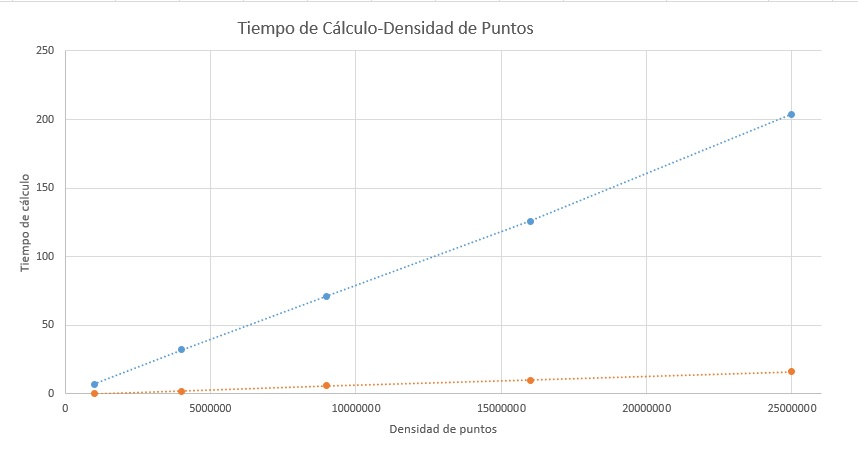
\includegraphics[width=15 cm]{T-Densidad_de_Puntos.jpg}				
\caption{Relación entre el tiempo de cálculo y la densidad de puntos para 1000 pasos temporales. La línea naranja representa el tiempo de ejecución en el device y la azul el tiempo de ejecución en el host. En ambas series de datos se ha representado la recta obtenida tras hacer una regresión lineal. Los valores de las pendientes obtenidos son 8.2 $\pm 0.2 \cdot 10^{-6}$ para la CPU y 6.52 $\pm 0.16 \cdot 10^{-7}$ para la GPU.}
\label{fig:t-densidad_de_puntos}
\end{figure}
\noindent









\section{Conclusiones}


En el presente documento se han resuelto las ecuaciones de Maxwell en $\mathbb R^{2}$ utilizando dos algoritmos desarrollados en CUDA, diseñados para realizar cálculos en procesador y tarjeta gráfica. Con ellos se ha determinado que, con los componentes utilizados (procesador i7-6700K  a una velocidad máxima de 4.2 Gigaherzios y tarjeta gráfica GTX 1070), se obtiene una ganancia en tiempo de cálculo de aproximadamente un órden de magnitud. Con las regresiones lineales de las secciones \ref{Subsection:Variacion pasos temporales}, \ref{subsection: Variacion densidad de puntos} podemos determinar que es especialmente útil el uso de GPUs a la hora de resolver problemas donde se realizan numerosos cálculos de matrices de forma reiterada ya que al aumentar el número de pasos se obtiene una pendiente mucho mayor en el tiempo de cálculo del algoritmo implementado en CPU, siendo esta pendiente mucho menos acusada en el algoritmo implementado en GPU.

Estos resultados son una muestra de las ventajas de aprender a utilizar la paralelización que nos ofrecen las GPUs a la hora de desarrollar soluciones de problemas con el cálculo de matrices, pudiendo llegar a realizar lo que antes requería una noche, en una hora.

\newpage

\appendix
\section{Datos y errores}\label{aped.A}
\subsection{Errores}
Para la propagación de errores se ha utilizado la expresión:

\begin{equation}
    \Delta f(a_i)=\sqrt{\sum_{i=1}^n (\frac{\delta f(a_i)}{\delta a_i} \cdot \Delta a_i)^2}
\end{equation}

\subsection{Datos}
\begin{table}[H]
    \centering
    \begin{tabular}{|r|c|c|c|}
    \hline
        \multicolumn{4}{ |c| }{CPU} \\ \hline
    Pasos Temporales &  $t_\text{CPU}$ ($\pm \SI{0.001}{\second}$) & $t_\text{CPU}$ ($\pm \SI{0.001}{\second}$) &  $t_\text{CPU}$  ($\pm \SI{0.001}{\second}$)\\ \hline \hline
     10    & 1.964 & 1.965 & 1.983  \\ \hline
     100   & 19.270 & 19.300 & 19.400  \\ \hline
     1000  & 209.483 & 210.762 & 206.966  \\ \hline
     10000 & 2169.530 & 2139.410 & 2139.820  \\ \hline
    \end{tabular}
    \caption{Ejecución en CPU con una densidad de puntos de 25 millones}
\end{table}


\begin{table}[H]
    \centering
    \begin{tabular}{|r|c|c|c|}
    \hline
        \multicolumn{4}{ |c| }{GPU} \\ \hline
    Pasos Temporales &  $t_\text{GPU}$ ($\pm \SI{0.001}{\second}$) & $t_\text{GPU}$ ($\pm \SI{0.001}{\second}$) &  $t_\text{GPU}$  ($\pm \SI{0.001}{\second}$)\\ \hline \hline
     10    & 0.165   & 0.167 & 0.164  \\ \hline
     100   & 1.638  & 1.632 & 1.630  \\ \hline
     1000  & 16.388 & 16.431 & 16.371  \\ \hline
     10000 & 168.697 & 167.173 & 169.841  \\ \hline
    \end{tabular}
    \caption{Ejecución en GPU con una densidad de puntos de 25 millones}
\end{table}


\begin{table}[H]
    \centering
    \begin{tabular}{|r|c|c|c|}
    \hline
        \multicolumn{4}{ |c| }{CPU} \\ \hline
    Densidad de puntos &  $t_\text{GPU}$ ($\pm \SI{0.001}{\second}$) & $t_\text{GPU}$ ($\pm \SI{0.001}{\second}$) &  $t_\text{GPU}$  ($\pm \SI{0.001}{\second}$)\\ \hline \hline
     $10^6 $         & 7.729   & 7.612 & 7.675  \\ \hline
     $4\cdot 10^6$   & 35.557  & 35.019 & 35.500  \\ \hline
     $9\cdot 10^6$   & 71.978 & 72.406 & 72.770  \\ \hline
     $16\cdot 10^6$  & 126.000 & 126.994 & 125.917  \\ \hline
     $25\cdot 10^6$  & 209.483 & 210.762 & 206.996  \\ \hline
    \end{tabular}
    \caption{Ejecución en CPU para un número de 1000 pasos temporales}
\end{table}


\begin{table}[H]
    \centering
    \begin{tabular}{|r|c|c|c|}
    \hline
        \multicolumn{4}{ |c| }{GPU} \\ \hline
    Densidad de puntos &  $t_\text{GPU}$ ($\pm \SI{0.001}{\second}$) & $t_\text{GPU}$ ($\pm \SI{0.001}{\second}$) &  $t_\text{GPU}$  ($\pm \SI{0.001}{\second}$)\\ \hline \hline
     $10^6 $         & 0.638   & 0.643 & 0.639  \\ \hline
     $4\cdot 10^6$   & 2.438  & 2.471 & 2.432  \\ \hline
     $9\cdot 10^6$   & 5.573 & 5.560 & 5.614  \\ \hline
     $16\cdot 10^6$  & 9.853 & 9.779 & 9.785  \\ \hline
     $25\cdot 10^6$  & 16.388 & 16.431 & 16.371  \\ \hline
    \end{tabular}
    \caption{Ejecución en GPU para un número de 1000 pasos temporales}
\end{table}



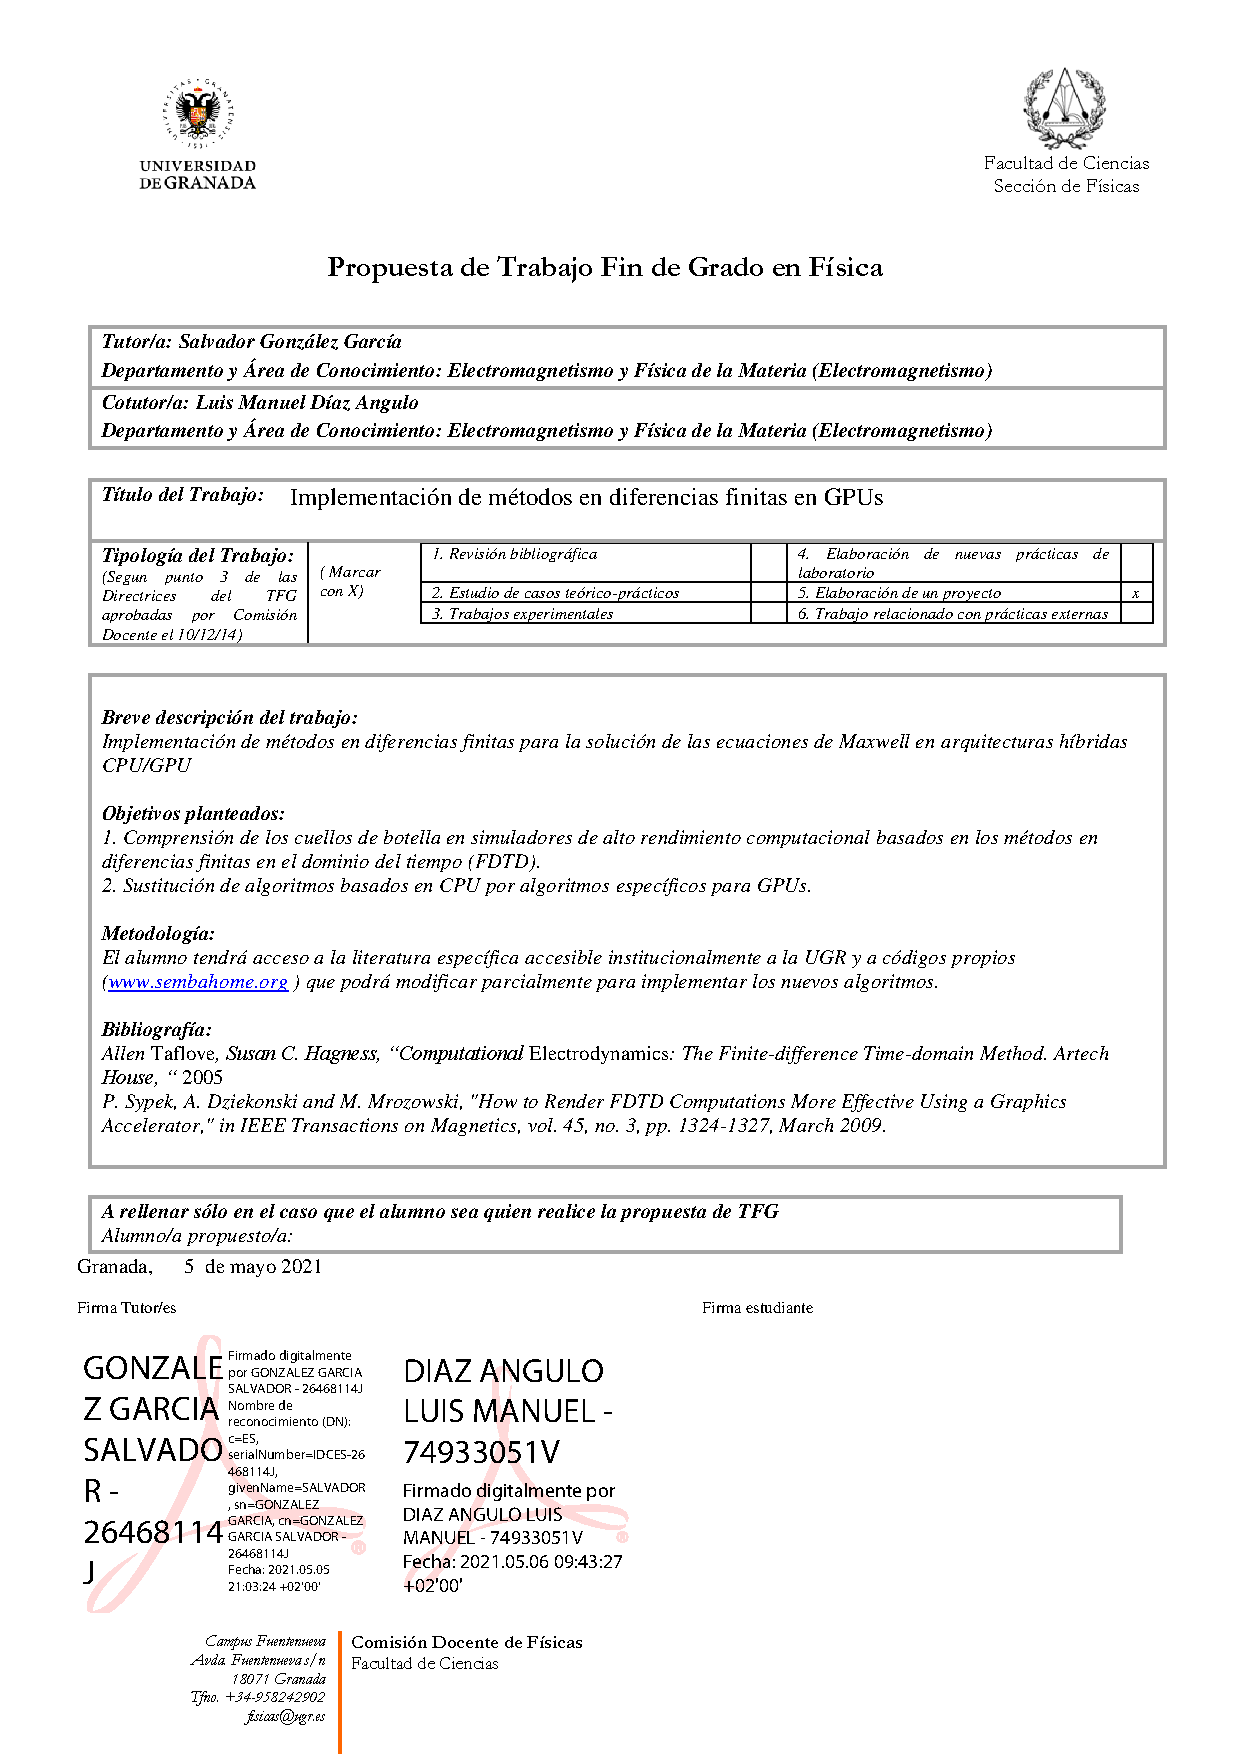
\includepdf[pages=-]{EFM-14.pdf}

% Referencias %%%%%%%%%%%%%%%%%%%%%%%%%%%%%%%%%%%%%%%%%%%%%%%%%%%%%%%%%%%%%%%%%
\newpage

\addcontentsline{toc}{section}{Referencias} % Elige según idioma
%\addcontentsline{toc}{section}{References} % Elige según idioma

\begin{thebibliography}{100}

\bibitem{Houle2020}
  Jennifer E~Houle and Dennis M~Sullivan, \\
  {\em Electromagnetic simulation using the FDTD method with Python}, \\
  IEEE PRESS WILEY, 2020.
  
  \bibitem{Taflove2005}
  Allen Taflove and Susan C~Hagness, \\
  {\em Computational electrodynamics. The Finite-Difference Time-Domain Method}, \\
  ARTECH HOUSE, 2005.

\bibitem{web}
 Nvidia documentation, \\
 \href{https://docs.nvidia.com/cuda/cuda-c-programming-guide/index.html}{https://docs.nvidia.com/cuda/cuda-c-programming-guide/index.html}
 
   \bibitem{Taflove1991}
  D.~ S.~ Katz, M.~ J.~ Piket-May, A.~ Taflove, K.~ R.~ Umashankar \\
  {\em FDTD Analisys of Electromagnetic Wave Radiation from Systems Containing Horn Antennas}, \\
  IEEE TRANSACTIONS ON ANTENNAS AND PROPAGATION, VOL.39, NO. 8, AUGUST 1991.

   \bibitem{Goorjian1991}
  P.~ M.~ Goorjian, P.~  M.~ Goorjian, A.~ Taflove \\
  {\em Direct time integration of Maxwell's equations in nonlinear dispersive media for propagation and scattering of femtosecond electromagnetic solitons}, \\
  Optics letters 1991.
  
     \bibitem{Taflove1998}
  S.~ C.~ Haness, A.~ Taflove, J.~ E.~ Bridges \\
  {\em Two-Dimensional FDTD Analisys of a Pulsed Microwave Confocal System for Breast Cancer Detection: Fixed-Focus and Antenna-Array Sensors}, \\
  IEEE TRANSACTIONS ON BIOMEDICAL INGINEERING , VOL 45, NO 12. DECEMBER 1998.

     \bibitem{Taflove2002}
  J.~ J.~ Simpsom, A.~ Taflove\\
  {\em Two-Dimensional FDTD Model of Antipodal Elf Propagation and Schumann Resonance on Earth}, \\
  IEEE ANTENAS AND WIRELESS PROPAGATION LETTERS, VOL.1 2002.

   
%\ \bibitem{conferencia}
%\   F.~Wilczek, \\
%\   {\em A long view of particle physics}, \\
%\   Proceedings of the 25th Solvay Conference on Physics, p. 210-249, \\  
%\   Brussels, Belgium, October 19-25, 2011.
%\ 
%\ \bibitem{charla}
%\   D.~Gross, \\
%\   {\em Quantum Field Theory: Past, Present and Future}, \\
%\   Talk at the Conference in Honour of the 90th Birthday of Freeman Dyson, \\
%\   Institute of Advanced Studies, Singapore, August 26-29, 2013.
%\ 
%\ \bibitem{libro}
%\   M.~E. Peskin and D.~V. Schroeder, \\
%\   {\em An Introduction to Quantum Field Theory}, \\
%\   Addison-Wesley, 1995.
%\   
%\ \bibitem{tesis}
%\   M.~R.~Chala, \\
%\   {\em Collider Signatures of a Non-Standard Higgs Sector}, \\
%\   PhD Thesis, Universidad de Granada, 2014.
%\ 
%\ \bibitem{web}
%\  Particle Physics News and Resources, \\
%\  \href{http://www.interactions.org/}{http://www.interactions.org/}
 
\end{thebibliography}



\end{document}


